\documentclass[11pt,a4paper]{article}
\usepackage[utf8]{inputenc}
\usepackage[T1]{fontenc}
\usepackage{amsmath}
\usepackage{amsfonts}
\usepackage[scale = 0.8]{geometry}
\usepackage{amssymb}
\usepackage{graphicx}
\usepackage{pdfpages}
\usepackage{hyperref}
\usepackage[round]{natbib}
\bibliographystyle{unsrtnat}
\usepackage{float}
\usepackage{subfig}
\usepackage{comment}
%\setlength{\parindent}{0pt}
\title{Melting or dissolving of vertical ice face into saline water}
\author{Yao Gahounzo\\[1cm]{\small Advisor: Dr. Michal Kopera}}

% insert month and year of your thesis, only:
\date{October 4, 2021}

\begin{document}
	
	%\maketitle
	
	\begin{titlepage} % Suppresses displaying the page number on the title page and the subsequent page counts as page 1
	\newcommand{\HRule}{\rule{\linewidth}{0.5mm}} % Defines a new command for horizontal lines, change thickness here
	
	\center % Centre everything on the page
	
	%------------------------------------------------
	%	Headings
	%------------------------------------------------
	
	\textsc{\LARGE BOISE STATE UNIVERSITY}\\[1.5cm] % Main heading such as the name of your university/college
	
	\textsc{\Large Computing PhD}\\[0.5cm] % Major heading such as course name
	
	\textsc{\large Computational Math Science and Engineering}\\[2cm] % Minor heading such as course title
	
	%------------------------------------------------
	%	Title
	%------------------------------------------------
	
	\HRule\\[0.4cm]
	
	{\huge\bfseries Melting or dissolving of vertical ice face into saline water}\\[0.4cm] % Title of your document
	
	\HRule\\[1.5cm]
	
	%------------------------------------------------
	%	Author(s)
	%------------------------------------------------
	
	\begin{minipage}{0.4\textwidth}
		\begin{flushleft}
			\large
			\textit{Author}\\
			Yao \textsc{Gahounzo} % Your name
		\end{flushleft}
	\end{minipage}
	~
	\begin{minipage}{0.4\textwidth}
		\begin{flushright}
			\large
			\textit{Advisor}\\
			Dr. Michal \textsc{Kopera} % Supervisor's name
		\end{flushright}
	\end{minipage}
	
	%------------------------------------------------
	%	Date
	%------------------------------------------------
	
	\vfill\vfill\vfill % Position the date 3/4 down the remaining page
	
	{\large\today} % Date, change the \today to a set date if you want to be precise
	
	%------------------------------------------------
	%	Logo
	%------------------------------------------------
	
	%\vfill\vfill
	%\includegraphics[width=0.2\textwidth]{placeholder.jpg}\\[1cm] % Include a department/university logo - this will require the graphicx package
	 
	%----------------------------------------------------------------------------------------
	
	\vfill % Push the date up 1/4 of the remaining page
	
    \end{titlepage}
	
	\section{Introduction and  Background}
	
	%The heat and freshwater exchange at the ice-ocean interface is the primary driver of creating new water masses. The Antarctic ice shelves either melt or dissolve depending on the seawater temperature.
	
	Ocean circulation leads to ice ablation in different geophysical conditions: ice shelves, glaciers, and ocean ice. The ablation is referred to as the thermodynamics of ice loss controlled by phase change into the ocean depending on the ocean and ice temperatures and composition \citep{malyarenko2020synthesis}. The ablation can be categorized into two thermal regimes depending on the ocean temperature and ice freezing temperature: melting or dissolution. The ice melting occurs due to the turbulent transport of salt and heat to the ice face \citep{gayen2016simulation}. It also occurs when the seawater is significantly warm.
	
    In contrast, the dissolution (phase change from solid to liquid) of ice occurs when the seawater temperature is below the melting temperature of $O^{\circ}$C \citep{mcphee1987dynamics, nicholls2012ocean, malyarenko2020synthesis}. At a low temperature, such as under the Oceanic Antarctic condition where the sea surface temperature is almost $O^{\circ}$C, the dissolution is controlled essentially by transfer of solute to the ice-ocean interface (Rignot and Jacobs2002, Payne et al. 2004, \cite{gayen2016simulation}). The dissolution rate greatly depends on the salt supply, which allows the temperature at the interface to be significantly lower than the freezing temperature of ice. When the dissolution occurs, the interface salinity gradient is non-zero \citep{kerr2015dissolution}. The ablation rate is also affected by the buoyancy or shear turbulent flux regimes; these regimes are defined based on the flow velocity within the boundary layer \citep{wells2008geophysical}. The dissolution and the melting of ice take place within the boundary layer next to the ice ocean. Hence, its knowledge is essential in predicting the melting rate and the future rise of seawater.
	
	The thermodynamic models of ice-ocean interaction are commonly described via the three equation formulation \citep{holland1999modeling}, where the conservation of heat and salt plays a vital role in predicting the interface temperature, salinity, and dissolution rate. The salinity is dependent on temperature and pressure at the interface. According to \cite{malyarenko2020synthesis}, although salt and heat conservation are currently widespread in ocean models, several terms are still not well constrained by observations. The coefficients used in the parameterization of heat, salt transfer from the far-field to the ice-ocean interface show the greatest dispersion. A lack of observations near the ice face introduces uncertainty in understanding the governing physical processes and leads to significant uncertainties regarding how critical processes are modeled \citep{malyarenko2020synthesis}.
	
	\cite{jenkins2010observations} conducted measurements with an autonomous underwater vehicle near the Pine Island Glacier to understand the dissolution processes and the melting at the ice shelves. They provided a detailed and spatially complete set of observations from the water column near the ice cavity. However, these measurements are very challenging for the flow field near the ice-ocean interface. Only the result from laboratory experiments on ice melting under oceanic conditions is available.
	
	The recent work of \cite{wells2011melting} analyzed the thermal and compositional boundary layer structure during the melting and dissolution. They determined the condition for the transition between the melting and dissolving regimes. However, another study pointed out that their analysis can not predict the dissolution or melting of large bodies of ice, especially in the polar ocean, because of turbulence that occurs from the connective flow after a vertical distance of 10-20 cm. \cite{gayen2016simulation}, in their work, also analyzed the structure of the boundary layer and concluded that it influences the dissolution velocity. Their results showed that the dissolution velocity is smaller due to a ticker thermal boundary layer in the laminar regime. However, dissolution velocity and temperature at the interface increase rapidly with a height from the bottom in the transition region.
    
    
    The simulation performed in this work follows the work done by \cite{gayen2016simulation} with some modification on the physical assumption using a spectral method or continuous Galerkin (CG) method in one dimension. The backward differentiation formula (BDF3) method is used for the time integration. The same ice-ocean properties and parameters have been used in our simulation to investigate the temperature and salinity profiles at the interface. In what follows, we described the two thermal regimes, melting and dissolution, followed by the governing equation that described the ocean system. The remaining sections of this work contain some test cases to verify the correctness of the CG methods followed the ice-ocean simulations results and conclusion
	
	
	\section{Thermal regimes}
	
	The ablation of ice releases melts of different compositions into the ocean. The difference in density of freshwater and ocean can be driven by convection in the ocean, which enhances heat and mass transfer from seawater and hence the rate of ablation. The ablation is a process that allows ice to lose mass by phase change. The phase change during the dissolution occurs to maintain chemical equilibrium at the ice face, while the phase change during melting is governed by heat transfer. Based on the previous studies \citep{wells2011melting, kerr2015dissolution}, the difference between melting and dissolving is illustrated through temperature and salinity profiles in the boundary layer.
	
	\begin{figure}[H]
		
		\centering
		\subfloat[\centering Dissolution: driven by slat transfer]{{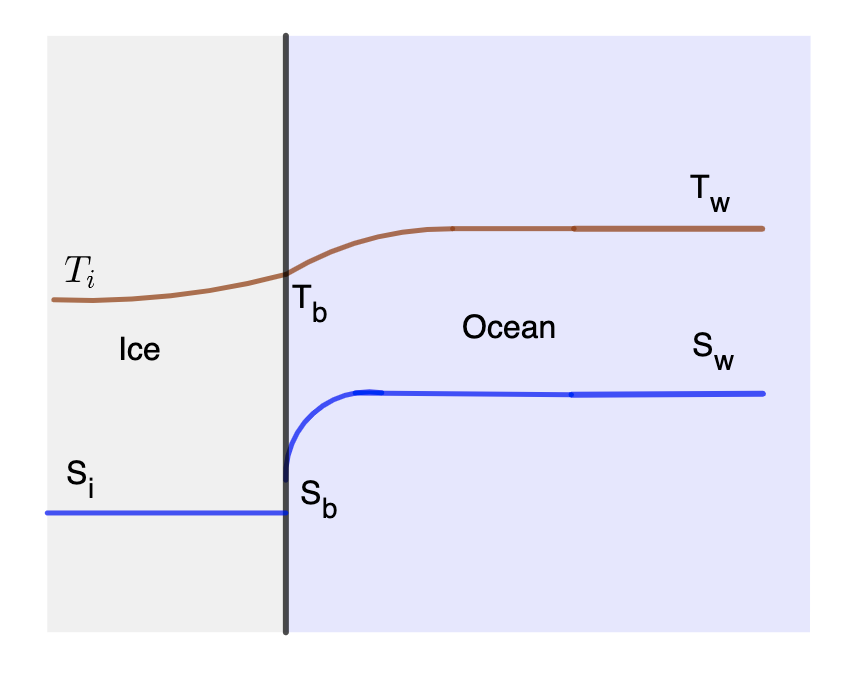
\includegraphics[width=8cm]{dissolution1.png} }}%
		\label{fig:4a}
		\subfloat[\centering Melting: driven by heat transfer]{{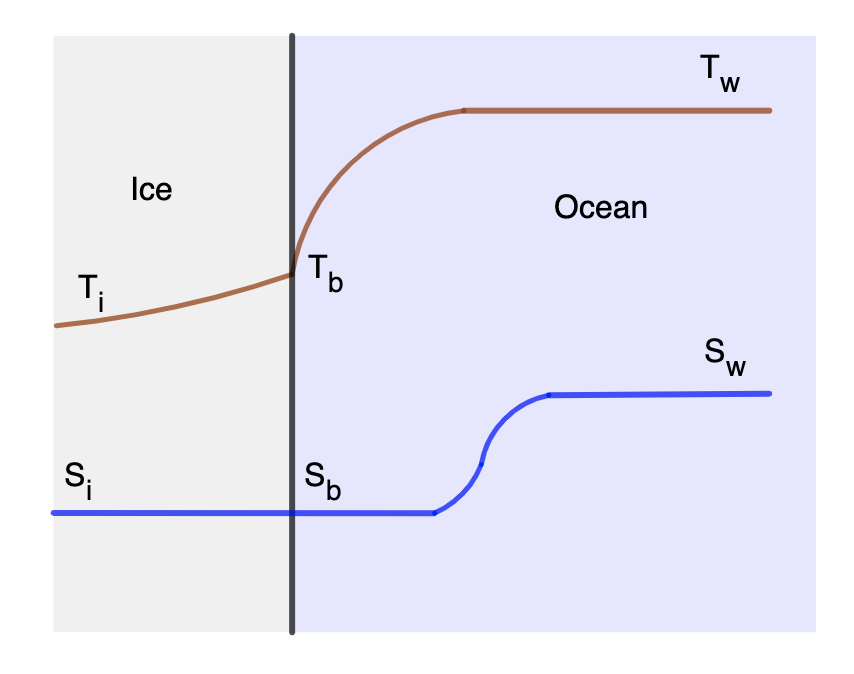
\includegraphics[width=8cm]{melting1.png} }}%
		\label{fig:4b}
		
		\label{fig:4}
		
		\caption{Schematic illustration of (a) dissolving and (b) melting of ice into saline water. The red line shows the temperature profile while the blue line represents the salinity profiles.}
	\end{figure}


	During the dissolution, a more significant diffusive salt flux inside the boundary layer leads to a larger salinity at the interface, depressing the freezing point temperature \citep{gayen2016simulation}. The heat transfer rate through the molecular sublayer can be two orders of magnitude higher than the salt transfer rate \citep{mcphee1987dynamics,malyarenko2020synthesis}. Therefore, salt transfer plays a limiting role in the rate of phase change. Alternatively, during the melting, the phase change is limited by how fast the heat is transferred from the ocean to the ice face because the rate of phase change is unaffected by how quickly salt can be transferred \citep{malyarenko2020synthesis}. During the dissolution, the ice face salinity gradient is non-zero \citep{kerr2015dissolution}; the ambient salinity differs from the interface salinity, and the interface temperature is below the freezing point temperature of the ice in pure water.
	
	The meltwater release is sufficiently rapid during the melting for a freshwater layer to develop immediately adjacent to the interface. During this process, only the temperature profile shows an appreciable gradient at the interface. Therefore, the melting rate is limited by heat transfer. The thermal regime determines whether the ice is dissolving or melting and impacts the structure of the ocean layer near the ice face.
	
	\section{Governing Equations}
	
	Most of the 3-D ocean circulation simulations use the Navier-stokes equations under the Boussinesq approximation. These equations are written as follows
	
	\begin{align}
		\nabla\cdot\mathrm{u} &= 0,\\
		\dfrac{D\mathrm{u}}{Dt} & = -\dfrac{1}{\rho_0}\nabla p + \nu\nabla^2\mathrm{u} - \dfrac{\Delta\rho}{\rho_0}g\mathbf{k},\\\label{eq:e3}
		\dfrac{D\mathrm{T}}{Dt} & = \kappa_T\nabla^2\mathrm{T} ,\\ \label{eq:e4}
		\dfrac{D\mathrm{S}}{Dt} & = \kappa_S\nabla^2\mathrm{S} ,\\ 
		\Delta\rho &=\rho_0\left[ \beta(S-S_w) - \alpha(T-Tw)\right].
	\end{align}

	where $\mathbf{u} = (u,v,w)$ is the flow velocity, $\mathrm{p}$ pressure, $T$ is the temperature with $T_w$ the far-field temperature and $S$ is the salinity with $S_w$ the far-field salinity. The density is $\mathrm{\rho}$ with $\rho_0$ the reference density and $\Delta \rho = \rho-\rho_0$. $\nu, \kappa_T$, and $\kappa_S$  the kinematic velocity, thermal diffusivity, and salinity diffusivity of the saline water respectively, $\alpha$  the coefficient of thermal expansion, and $\beta$ the coefficient of haline contraction.
	
	\begin{figure}[H]
	    \centering 
	    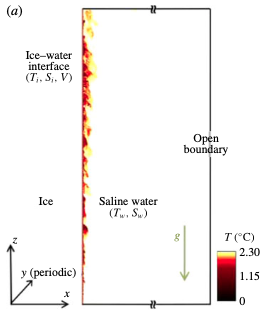
\includegraphics[width=8cm]{domain}
	    \caption{Schematic of the simulation domain \cite{gayen2016simulation}}
	\end{figure}
	
	At the left-hand side of the domain, the vertical ice face of height $H$ is placed and and it is in contact with seawater at initial temperature $T_w$ and salinity $S_w$. The right-hand side of the domain has an open boundary condition.
	
	In this work, we restrained our models into one dimension. The focus is on the temperature and salinity profile at the ice-ocean interface, so the simulation considers only the equations $(\ref{eq:e3})$ and $(\ref{eq:e4})$ that describe the diffusion of temperature and salinity. The equations $(\ref{eq:e3})$ and $(\ref{eq:e4})$ in one dimension becomes
	
	\begin{eqnarray}
		\label{eq:6}
		\dfrac{\partial\mathrm{T}}{\partial t} & = \kappa_T\dfrac{\partial^2T}{\partial x^2} ,\\[0.3cm] 
		\label{eq:7}
		\dfrac{\partial\mathrm{S}}{\partial t} & = \kappa_S\dfrac{\partial^2S}{\partial x^2} . 
	\end{eqnarray}
	
	
	\section{Vertical ice face}
	
	A meltwater plume rising along the ice face sustains convection, and the plume volume flux grows with height \citep{jenkins2011convection}. The ablation rate depends not only on the thermal and salt diffusivities but also on the structure of the boundary layer. In the laminar regime, the ablation rate is lower due to the thicker thermal boundary layer. At the same time, within the transition region, the interface temperature and ablation rate increase rapidly with the rising plume \citep{gayen2016simulation}. In the works done by \cite{kerr2015dissolution} and \cite{gayen2016simulation}, where they considered vertical ice adjacent to the ocean, the dissolution rate is controlled by the buoyancy-driven, and it is independent of the depth and plume velocity. They have shown in their analysis that the ablation rate is 
	
	\begin{equation}
	    V = constant\times (T_w-T_L)^{1.34},
	\end{equation}
	
	which is consistent with the theory prediction. The authors also pointed out that when the ambient temperature exceeds $3-4^{\circ} C$ above the freezing point temperature, a transition into turbulent melting is approached, and the interface temperature is overestimated.
	
	Another theoretical scaling for both vertical and horizontal boundaries suggests the existence of the second regime of turbulent natural convection at high Rayleigh numbers ($R_a> 10^{16}$). During that regime, the thickness of the inner laminar boundary layer near the ice face is controlled by shear production rather than convective production of turbulence \citep{grossmann2000scaling, wells2008geophysical,kerr2015dissolution,gayen2016simulation}. The transition between buoyancy-driven and shear-driven regimes is predicted to happen at more significant Rayleigh number $R_a \thicksim 10^{16}$ for thermal convection in air. However, for compositional convection during ice dissolution, the transition is predicted to occur at Rayleigh number $R_a \thicksim 10^{21}$ \citep{kerr2015dissolution,gayen2016simulation}.

    \section{Boundary conditions}
    
    	The freezing point of seawater is a weakly nonlinear function of salinity and a linear function of pressure \citep{millero1978freezing}. However, a linearized form is used in most of the studies to simplify the solution to the three-equations system. The relationship between the temperature and salinity at the ice-ocean interface, $T_b$ and $S_b$ is given by
		
		\begin{equation}
			\label{eq:1}
			T_b = aS_b+b+cp_b
		\end{equation}
		
		where $p_b$ is the pressure at the interface and $a,b,c$ are constants.
		
		The conservation of heat at the interface requires that the divergence of the heat flux balances the source of latent heat resulting from ablation at the interface
		
		\begin{eqnarray}
			\label{eq:2}
			Q_i^T - Q_w^T = Q_{latent}^T
		\end{eqnarray}
		
		where the latent heat is given by $$Q_{latent}^T = -\rho_wVL_i,$$ with $\rho_wV$ representing the mass of ice that melted per unit time. $V$ is the melt rate and $\rho_w$ is the ocean density. $Q_i^T$ is the heat flux through ice and $ Q_w^T$ is the heat flux in boundary layer.
		
		Similary, the conservation of salinity is given by
		
		\begin{equation}
			%\label{eq:3}
			Q_i^S - Q_w^S = Q^S_{brine}
		\end{equation}
		
		where $Q_{brine}^S = \rho_wV(S_i-S_b)$ is the salt flux necessary to maintain the interface salinity at $S_b$, $Q_i^S$ is the salt flux through ice and $Q_w^S$ is the salt flux in boundary layer. The diffusive flux of salt into the ice, $Q_i^S$ and $S_i$ are considered to be equal to zero.  The salt conservation becomes 
		
		\begin{equation}
			\label{eq:4}
			Q_w^S = \rho_wVS_b.
		\end{equation}

		The diffusive fluxes are expected to be proprotional to their respective gradients, so
		
		\begin{align}
			\label{eq:tq1}
			Q_i^T &= -\rho_ic_i\kappa_i^T\dfrac{\partial T_i}{\partial x}\bigg|_b\\		
			\label{eq:tq2}	
			Q_w^T& = -\rho_wc_w\kappa_w^T\dfrac{\partial T_w}{\partial x}\bigg|_b\\
			\label{eq:tq3} 
			Q_w^S& = -\rho_w\kappa_w^s\dfrac{\partial S_w}{\partial x}\bigg|_b
		\end{align}
	
	
		$c_i, c_w$ are the specific heat capacities of ice and ocean, $\kappa_i^T, \kappa_w^T$ are the thermal diffusivities of ice and ocean, and $\rho_i$ is the ice density.
		
		In equation $(\ref{eq:tq1})$, $\rho_i, c_i, \kappa_i^T$ are assumed to be constants and we need to estimate the temperature gradient at the ice-ocean interface. In equation $(\ref{eq:tq2})$, $\rho_w, c_w,$ are assumed to be constants and we need a good paramerization of  products of the diffusivities and the gradients at the ice-ocean interface.
		
		In the case of a laminar boundary layer, the temperature and salinity would vary linearly between the interface and the mixed temperatures (seawater temperatures)\cite{holland1999modeling}, so we have
		
		\begin{equation}
			Q_w^T = -\rho_wc_w\kappa_w^T\dfrac{T_b-T_w}{h},
		\end{equation}
	
		where $h$ is the boundary layer thickness. Turbulence in the boundary layer create a nonlinear temperature profile and variable diffusivity, but we parameterize this complicated situation by introducing a nondimensional empirical parameter Nusselt number, $N_u$, with value greather than one, so that
		
		\begin{equation}
			Q_w^T = -\rho_wc_w\left(\dfrac{N_u\kappa_w^T}{h}\right)\left(T_b-T_w\right).
		\end{equation}
		
		The first quantity in brackes has dimensions of velocity, so we refer it as thermal exchange velocity $\gamma_T$, then 
		
		\begin{equation}
			Q_w^T = -\rho_wc_w\gamma_T(T_b-T_w).
		\end{equation}
	
		Similarly by following the previous steps we obtain
		
		\begin{equation}
			Q_w^S = -\rho_w\gamma_S(S_b-S_w),
		\end{equation}
		
		where $\gamma_S$ is reffered as salinity exchange velocity. The exchange velocities parameterization must consider both turbulent effects in the boundary layer and diffusive effects in a thin, viscous sublayer adjacent to the interface. Such parameterization is then
		
		\begin{equation}
			\label{eq:gT}
			\gamma_{T} = \dfrac{u_*}{2.12\ln\bigg(\frac{u_*h}{\nu}\bigg)+12.5 Pr^{2/3}-9}
		\end{equation}
		
		
		and
		
		\begin{align}
			\label{eq:gS}
			\gamma_{S} = \dfrac{u_*}{2.12\ln\bigg(\frac{u_*h}{\nu}\bigg)+12.5 Sc^{2/3}-9},
		\end{align}
		 
		
		where $Pr = \dfrac{\nu}{\kappa_w^T}$ is the Prandtl number and $Sc =  \dfrac{\nu}{\kappa_w^S}$ is the Schmidt number, $\nu$ is the kinematic viscosity. The friction velocity $u_*$ at the interface is defined in terms of a dimensionless drag coefficient $c_d$ and velocity $U_M$ of the layer next to the ice face by
		
		$$u_*^2 = c_d U_M^2.$$
		
		The exchange velocities can be either assumed constant or as function dependence on friction velocity as described in $(\ref{eq:gT})$ and $(\ref{eq:gS})$.
		
		
		We close the three-equation formulation by estimating the temperature gradient in the ice. The approximation we would require solving the heat transport equation in the ice
		
		\begin{equation}
			\label{eq:ice1}
			\dfrac{\partial T_i}{\partial t} +U_i\cdot\nabla T_i = \kappa_i^T\nabla^2T_i.
		\end{equation}
		
		We assume that the vertical velocity is constant and equal to the melt rate and that the ice is in a steady state. The equation $(\ref{eq:ice1})$ 
		
		$$\dfrac{\partial^2 T_i}{\partial x^2} + \frac{V_i}{\kappa_i^T}\dfrac{\partial T_i}{\partial x} = 0, V_i = \frac{\rho_w}{\rho_i}V.$$
		
		Assuming that the solution is in the form $T(x) = e^{mx}$, the latter equation becomes 
		
		$$m^2+ \frac{V_i}{\kappa_i^T}m = 0,$$ this implies $m_1 = - \frac{V_i}{\kappa_i^T}, m_2 = 0.$
		
		The solution to the equation $(\ref{eq:ice1})$  is then 
		
		$$T_i(x) = c_1e^{m_1z}+c_2.$$
		
		Using the boundary conditions
		
		$$x = 0 \text{ (ice surface)}, T_i(0) = T_i$$
		$$x = -H_i \text{ (ice base)}, T_i(-H_I) = T_B$$ we obtained
		
		$$c_1 = \dfrac{T_i-T_b}{1-\exp(-m_1H_i)}, \quad c_2 = \dfrac{T_b-T_ie^{-m_1H_i}}{1-\exp(-m_1H_i)}$$
		
		Replacing $c_1, c_2$ in the expression of $T_i(x)$ and taking its derivative at the boundary we have
		
		\begin{equation}
			\label{eq:ice2}
			\dfrac{\partial T_i}{\partial x}\bigg|_b = \prod\cdot \dfrac{T_i-T_b}{H_i}
		\end{equation}
		
		where $\prod = \dfrac{\gamma}{e^{\gamma}-1}, \quad \gamma = -\dfrac{V_iH_i}{\kappa_i^T}.$
		
		The expression of $\prod$ can be simplified as 
		
		$$\prod = \dfrac{\rho_wH_i}{\rho_I\kappa_i^T}V,$$
		
		therfore, the equation $(\ref{eq:ice2})$ becomes
		
		\begin{equation}
			\label{eq:16}
			\dfrac{\partial T_i}{\partial x}\bigg|_b = \dfrac{\rho_wV}{\rho_i\kappa_i^T}\left( T_i-T_b\right).
		\end{equation}
	
		By using the approximation of the heat and salt gradient at the interface, we obtain the full three-equation formulation as
		
		\begin{align}
			T_b & = a S_b + b + cp_b\\
			c_iV\left(T_i-T_b\right) + c_w\gamma_T(T_w-T_b)& = VL_i\\
			\gamma_S(S_w-S_i) & = VS_i.
		\end{align}
	
		After some algebraic, we solve for $S_b$ and find that
		
		\begin{equation}
			AS_b^2 + BS_b + C = 0,
		\end{equation}
		
		where
		
	\begin{align*}
		A &= a(c_w\gamma_T-c_i\gamma_S),\\
		B &= -c_w\gamma_T(T_w-b-cp_b) + c_i\gamma_S(T_i-b-cp_b+aS_w)-\gamma_SL_i,\\
		C &= \gamma_SL_iS_w-c_i\gamma_SS_w(T_i-b-cp_b).
	\end{align*}
		
	The value of $V$ and $T_b$ is computed after computing $S_b$. To solve the diffusion equations $(\ref{eq:6})$ and $(\ref{eq:7})$ and determine the characteristics of the salinity and temperature, we revisited the conservation of salt and heat at the interface. The boundary conditions at the ice-ocean interface are define as follows 
	
	\begin{equation}
		\label{eq:eq10}
		\dfrac{\partial T}{\partial x}\bigg|_b = \dfrac{\rho_iL_i}{\rho_wc_w\kappa_T}V
	\end{equation}
	
	\noindent for the temperature and 
	
	\begin{equation}
		\label{eq:eq11}
		\dfrac{\partial S}{\partial x}\bigg|_b = \dfrac{\rho_i}{\rho_w\kappa_S}S_bV
	\end{equation}
	
	\noindent for salinity.
	
	
	\begin{comment} 
	To solve the above equations and determine the characteristics of the salinity and temperature at the interface, three physical constraints have to be considered. The interface must be at the freezing point, heat and salt must be conserved at the interface during any phase change. The temperature at the interface is controlled by the salinity at the interface $S_b$, and the relation between these quantities is given by
	
	
	%The equations solved at the boundary are 
	
	\begin{equation}
		\label{eq:9}
		T_b = \lambda_1S_b + \lambda_2 + \lambda_3p_b,
	\end{equation} 
	
	\noindent  where $V$ is the melt rate, $\lambda_i, i=1,2,3$ are constants, $T_b$ and $p_b$ is the temperature and pressure at the ice-ocean interface respectively. The equation $(\ref{eq:9})$ is commonly used in ice-ocean interaction models. However, \cite{gayen2016simulation} used its simplified version in their work where they neglected the interface pressure over 1 m depth scale of the domain.
	
	The divergence of the heat flux balances the source of latent heat caused by dissolution at the ice-ocean interface gives
	
	\begin{eqnarray}
	 		\label{eq:2}
	 		\rho_ic_i\kappa_T^i\dfrac{\partial T}{\partial x}\bigg|_b - \rho_wc_w\kappa_T\dfrac{\partial T}{\partial x}\bigg|_b = -\rho_iL_iV
 	\end{eqnarray}
 	
 	$\rho_i, L_i$ is the density and latent heat of the ice, $\rho_w$ is the density of the seawater,$\rho_w$ and $c_w$ is the density and specific heat of the saline water, $c_i$ and $\kappa_T^i$ is the specific heat and thermal diffusivity of ice. The heat conduction within the ice is neglected and tha latter equation becomes

	\begin{equation}
		\label{eq:eq10}
		\dfrac{\partial T}{\partial x}\bigg|_b = \dfrac{\rho_iL_i}{\rho_wc_w\kappa_T}V.
	\end{equation}
    
    Similarly to the heat conservation, we obtain the conservation of salt by neglecting the diffusive salinity flux and the salinity in the ice, and this leads to
    
	\begin{equation}
		\label{eq:eq11}
		\dfrac{\partial S}{\partial x}\bigg|_b = \dfrac{\rho_i}{\rho_w\kappa_S}S_bV.
	\end{equation}
	
	\medskip
	
	 
	The parameters $\rho_i, c_i, \kappa_T, \kappa_S$, $\rho_w, c_w$ are assumed to be constants and the estimation of the temperature and salinity gradients at the ice-ocean interface are needed. 
	
	We need to find $V,T_b$, and $S_b$ at the interface. Their computation are based on the so-called diffusive three equations formulation. For more detail, we refer the reader to \cite{holland1999modeling}. Assuming that the boundary layer were laminar, the temperature (or salinity) would vary linearly between the interface and the mixed temperature (or salinity) and the melt rate, salinity and temperature at the boundary are computed as follows 
 	
 	\begin{eqnarray}
 	    T_b & = \lambda_1S_b + \lambda_2 + \lambda_3p_b,\\[0.3cm]
 	    -c_iV\left( T_i-T_b\right)+c_w\gamma_T(T_b-T_w) & = -V L_f,\\[0.3cm]
 	    -\gamma_S(S_b-S_w) & = V S_b.
 	\end{eqnarray}
 	
 	\medskip 
	
	After doing some algebraic we have
	\begin{equation}
		\label{eq:12}
		V = \gamma_S\left(\dfrac{S_w-S_b}{S_b}\right),
	\end{equation}
	
	\begin{equation}
		\label{eq:13}
		T_w-T_b = \dfrac{\gamma_S}{\gamma_T}\bigg[ \dfrac{L_i+c_i(T_b-T_i)}{c_w}\bigg]\left(\dfrac{S_w-S_b}{S_b}\right),
	\end{equation}

	\begin{equation}
		\label{eq:14}
		AS_b^2+BS_b+CS_w = 0,
	\end{equation}
	
	where
	
	$$A = \lambda_1\left(1-\dfrac{\gamma_S}{\gamma_T}\right), \quad B = -T_w-\dfrac{\gamma_S}{c_w\gamma_T}(L_i-c_iT_b)+(\lambda_2+\lambda_3p_b)\left(1-\dfrac{\gamma_S}{\gamma_T}\right)+\lambda_1\dfrac{\gamma_S}{\gamma_T}S_w,$$
	and
	
	$$C = \dfrac{\gamma_S}{c_w\gamma_T}(L_i-c_iT_i)+\lambda_1\dfrac{\gamma_S}{\gamma_T}(\lambda_2+\lambda_3p_b).$$
	
	$\gamma_T$ is the temperature exchange velocity, and $\gamma_S$ is the salinity exchange velocity that we assumed constants.
	
	\end{comment}
	
	The simulation domain consists of interval $0$ to $0.5$ m where $x = 0$ represent the ice-ocean interface. A second order Lagrange polynomial ($N=2$ is used with total number of 256 elements to subdivide the domain. The Courant-Friedricks-Lewy number is $1/(N+1)$.
	
	\section{Numerical method: Spectral method}
	
	A spectral method presents some advantages in ocean modeling, which involves the complex interaction of stratified flows with topography. The spectral element method offers a good convergence with elemental grid refinement or increasing in the order of interpolation polynomial \citep{ilicak2009non}. The method presents no significant numerical dissipation and provides geometrical flexibility, especially for problems in complex geometry. Another advantage is the scalability of its code in parallel machines
	
	Unlike the DNS method used by \cite{gayen2016simulation}, we used the CG method with the implicit time integration BDF3. As it was implemented to obtain the results in this study, a summary of the CG method is described using the following equation.
	
	\begin{equation}
	\label{eq:diff}
	    \dfrac{\partial q(x,t)}{\partial t} = \dfrac{\partial^2 q(x,t)}{\partial x^2},
	\end{equation}
	
	\noindent with either Neumann or Robin boundary conditions. We divide the problem domain $\Omega\in\mathbb{R}$ into $N_e$ elements
	
	$$\Omega = \bigcup_{i=1}^{Ne}\Omega_e.$$
	We create an approximation $q_N^{(e)}(x,t)$ to $q(x,t)$ within each element $\Omega_e$ using 
	
	\begin{equation}
	\label{eq:17}
	    q_N^{(e)}(x,t) = \sum_{j=1}^{M} \psi_jq_j^{(e)}(t),
	\end{equation}
	
	where $M$ is the number of nodes in the element, $\psi_j$ is a basis function, $q_j^{(e)}$ is the expansion coefficient and the superscript $^{(e)}$ denotes the element index.
	
	We expand both sides of equation $(\ref{eq:diff})$ using the approximation $(\ref{eq:17})$, multiplying with the basis function $\psi_i$ and integrate within each element 
	
	\begin{equation}
	    \int_{\Omega_e}\psi_i\dfrac{\partial q_N^{(e)}}{\partial t}d{\Omega_e} = \int_{\Omega_e}\psi_i\dfrac{\partial^2 q_N^{(e)}}{\partial^2 x}d{\Omega_e}
	\end{equation}
	
	Using integration by parts and divergence theorem in the right-hand-side we obtain
	
	\begin{equation}
	    \int_{\Omega_e}\psi_i\psi_jd{\Omega_e}\dfrac{d q_N^{(e)}}{dt} = \int_{\Gamma_e}\psi_i\dfrac{\partial q_N^{(e)}}{\partial x}d{\Gamma_e} - \int_{\Omega_e}\dfrac{d\psi_i}{dx}\dfrac{d\psi_j}{d x}d{\Omega_e}q_N^{(e)}
	    \label{eq:20}
	\end{equation}
	
	The first term on the right-hand side is used to apply the boundary conditions. Due to the continuity across element interfaces, the inter-element edges vanish when the direct stiffness summation is applied to the first term on the right-hand side.
	
	\begin{comment}
	\subsection{Neumann boundary conditions}
	    
	    The Neumann boundary condition is generally described as follows
		\begin{equation}
			\label{eq:neu}
				\dfrac{\partial q(x,t)}{\partial x}  = h(x), \quad x\in \partial \Omega.
		\end{equation}
		
		\noindent Applying the Neumann condition $(\ref{eq:neu})$, equation $(\ref{eq:20})$ becomes 
		
		\begin{equation*}
	    \int_{\Omega_e}\psi_i\psi_jd{\Omega_e}\dfrac{d q_N^{(e)}}{dt} = \int_{\Gamma_e}\psi_i h(x)d{\Gamma_e} - \int_{\Omega_e}\dfrac{d\psi_i}{dx}\dfrac{d\psi_j}{d x}d{\Omega_e}q_N^{(e)}
	    \end{equation*}
	    
	    \noindent In the matrix form, we get 
	    \begin{equation}
		    M_{ij}^{(e)}\dfrac{dq_j^{(e)}}{dt} = c^2B_j^{(e)} - c^2L_{ij}^{(e)}q_j^{(e)}.
		\end{equation}
	
	\subsection{Robin boundary condition}
	    
	    The general description of Robin boundary condition is given in below equation
	    
		\begin{equation*}
			\label{eq:4}
			\dfrac{\partial q(x,t)}{\partial x} + kq(x,t)  = g(x), \quad x\in \partial \Omega. 
		\end{equation*}
		
		\noindent Applying the above condition, equation $(\ref{eq:20})$ becomes
		
		\begin{align*}
		    \int_{\Omega_e}\psi_i\psi_jd{\Omega_e}\dfrac{d q_N^{(e)}}{dt}& = \int_{\Gamma_e}\dfrac{\partial}{\partial x}\big(\psi_i (g(x)\big) - k\dfrac{\partial}{\partial x}\big(\psi_iq(x,t))\big)d\Gamma_e- \int_{\Omega_e}\dfrac{d\psi_i}{dx}\dfrac{d\psi_j}{d x}d{\Omega_e}q_N^{(e)}\\[0.3cm]
		    \int_{\Omega_e}\psi_i\psi_jd{\Omega_e}\dfrac{d q_N^{(e)}}{dt}& = \int_{\Gamma_e}\dfrac{\partial}{\partial x}\big(\psi_i (g(x)\big)d\Gamma_e - k\int_{\Gamma_e}\dfrac{\partial}{\partial x}\big(\psi_iq(x,t))\big)d\Gamma_e - \int_{\Omega_e}\dfrac{d\psi_i}{dx}\dfrac{d\psi_j}{d x}d{\Omega_e}q_N^{(e)}\\
		\end{align*}
		
		In the matrix form we get 
		\begin{equation}
		    M_{ij}^{(e)}\dfrac{dq_j^{(e)}}{dt} = c^2B_j^{(e)} - c^2\left(kF_{ij}^{(e)} + L_{ij}^{(e)}\right)q_j^{(e)}.
		\end{equation}
		
	
	 The direct stiffness summation is applied to move from the element reference equation to the global equation.
	
	\end{comment} 
	
	\section{Results}
	
	We begin this section by presenting some convergence test cases for the CG method using both Neumann and Robin boundary conditions to validate the correctness of the code. It is followed by the temperature and salinity profile results at the ice-ocean interface and dissolution rate against variation in far-field salinity.
	
	\subsection{Ideal test for numerical verification}
	
	In order to verify the correctness of the CG method described in section 4, two simple ideal diffusion equations have been solved with Neumann 
	
	\begin{align*}
	    \dfrac{\partial\mathrm{q(x,t)}}{\partial t} & = \dfrac{\partial^2\mathrm{q(x,t)}}{\partial x^2}, \quad x\in [0,1]\\
	    \dfrac{\partial\mathrm{q}}{\partial x} & = 0, \quad x\in \{0,1\},
	\end{align*}
	
	where exact solution $ q(x,t) = \exp(-\pi^2t)\cos(\pi x)$. And with Robin boundary conditions 
	
	\begin{align*}
	    \dfrac{\partial\mathrm{q(x,t)}}{\partial t} & = \dfrac{1}{25}\dfrac{\partial^2\mathrm{q(x,t)}}{\partial x^2}, \quad x\in [0,3]\\
	    q(0,t) &= 0\\
        \dfrac{\partial\mathrm{q}}{\partial x}(3,t) &= -\dfrac{1}{2}q(3,t)\\
        q(x,0) &= 100\bigg(1-\dfrac{x}{3}\bigg)\\
	\end{align*}
	
	where exact solution 
	
	$$ q(x,t) = \sum_{n=1}^{\infty}\dfrac{200(3\nu_n-\sin(3\nu_n))}{3\nu_n^2(3+2\cos^2(3\mu_n))}\exp(-\nu_n^2t/25)$$
	
	with $\nu$ the nth positive solution to $\tan(3\nu) = -2\nu.$
	
	The tow-norms errors in the numerical and exact solutions are presented in the graph below
	
	%\begin{center}
	%    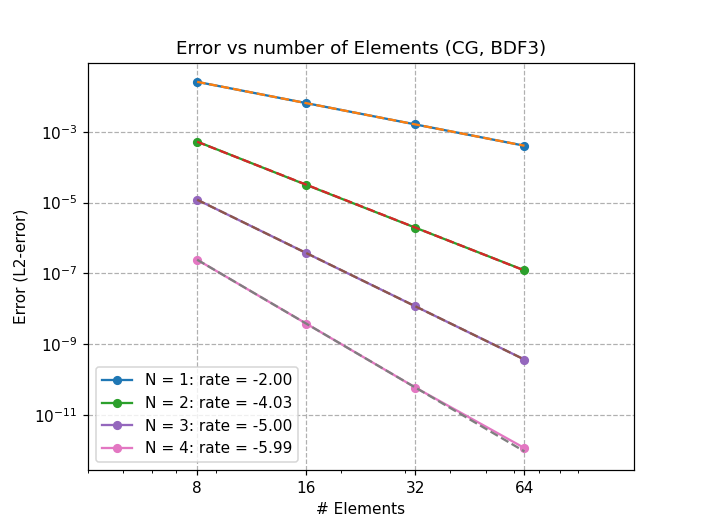
\includegraphics[width=12cm]{unitNeumann}
	%\end{center}
	
	\begin{figure}[H]
		
		\centering
		\subfloat[\centering Neumann BC]{{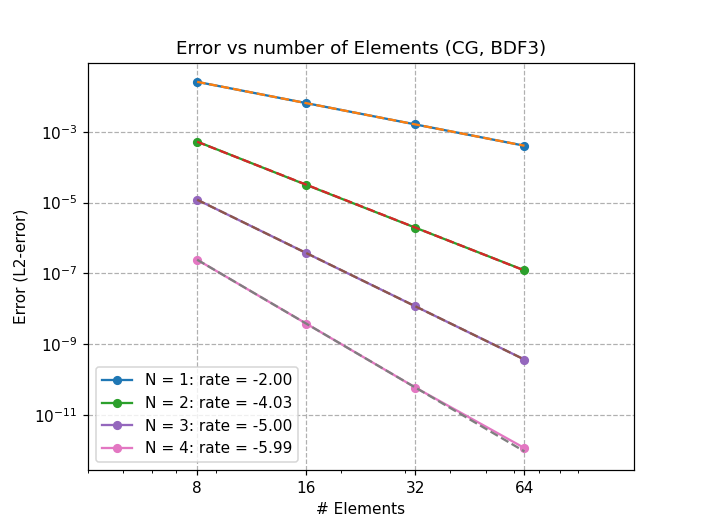
\includegraphics[width=8cm]{unitNeumann} }}%
		\label{fig:4a}
		\subfloat[\centering Robin BC]{{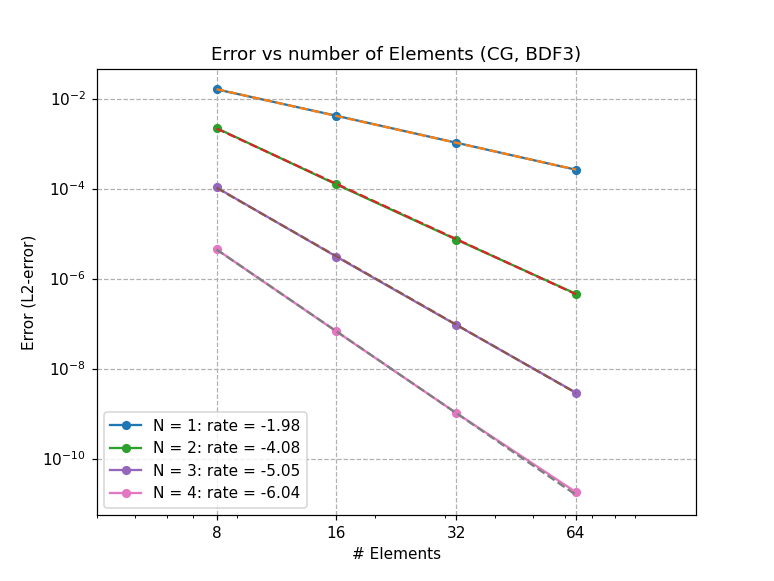
\includegraphics[width=8cm]{unitRobin.png} }}%
		\label{fig:4b}
		
		\label{fig:4}
	\end{figure}
	
	In both figure, the numerical method CG produces a very good accuracy and order of convergences. In both figures, the numerical method CG produces excellent accuracy and order of convergence. The convergence rates are approximately $N+1$, $N$ denotes the order of basis polynomial used in the numerical integration.\\
	
	\subsection{Temperature profile at the ice-ocean interface}
	
	The value of some physical constants has been used in solving the PDEs that described the thermal and salinity behaviors at the ice-ocean interface, the same as in Jenkins et al. (2001). The value of these constants is summarized in the table below.\\
	
	\begin{tabular}{ |p{8cm}||p{2cm}|p{3cm}|p{3cm}|}
		\hline
		\multicolumn{4}{|c|}{Model parameters and constants} \\
		\hline
		Parameter &Symbol&Units&Value\\
		\hline
		Salinity coefficient of freezing equation &a& $^{\circ}$C $psu^{-1}$&   $-5.73\times10^{-2}$\\
		Constant coefficient of freezing equation &b&  $^{\circ}$C  & $8.72\times 10^{-2}$\\
		Pressure coefficient of freezing equation& c&$^{\circ}$C $Pa^{-1} $& $-7.53\times10^{-8}$\\
		Latent heat of the ice    & $L_i$ & J $kg^{-1}$& $3.35\times 10^{5}$\\
		Thermal diffusivity& $\kappa_S$  & $m^2 s^{-1}$&$7.4\times 10^{-7}$\\
		Salinity diffusivity & $\kappa_T$  & $m^2 s^{-1}$   &$1.3\times 10^{-7}$\\
		Temperature of the far-field& $T_w$  & $^{\circ}$C & 2.3\\
		Salinity of the far-field&$S_w$& psu&  35  \\
		%Temperature at ice shelf surface& T_b& $^{\circ}$C & \\
		%Salinity at ice shelf surface & S_b& psu & \\
		Density of the ice & $\rho_i$& $kg m^{-3}$& 920\\
		Density of the seawater & $\rho_w$ & $kg m^{-3}$& 1000\\
		%Melt rate & V & m s^{-1}& \\
		Thermal exchange velocity & $\gamma_T$ & $m s^{-1}$& $5\times 10^{-3}$\\
		Salinity exchange velocity & $\gamma_S$ & $m s^{-1}$& $0.04\gamma_T$ \\
		Specific heat of saline water& $c_w$ & $J kg^{-1}K^{-1}$ & 3974.0\\
		Specific heat of ice & $c_i$ & $J kg^{-1} K^{-1}$ & 2009.0\\
		\hline
	\end{tabular}
    
    \bigskip 
    
    The main goal of this work is to investigate the behavior of temperature and salinity at the interface, and they affect the dissolution rate. The simulations are initialized with the far-field temperature, $T_w$, and salinity, $S_w$. In all the simulations for temperature and salinity profiles, the ambient salinity is set to be 35 psu.
	
	\begin{figure}[H]
	    
	    \centering 
	    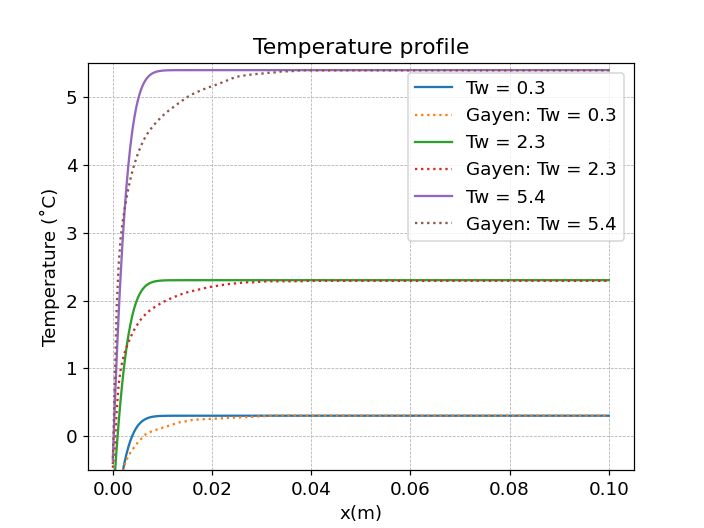
\includegraphics[width=12cm]{tempProfile}
	    \caption{Temperature profile}
	    \label{fig:2}
	\end{figure}
	
	
	Temperature profiles obtained from this study are shown in figure $\ref{fig:2}$ for three different far-field temperatures at constant salinity ($S_w = 35$ psu) along with those in \citet{gayen2016simulation}. The temperature increases from the mid-depth at the ice face through the plume to a steady value. The decrease in ambient temperature affects the temperature profile at the boundary. The discrepancies observed in the current results and those in \citet{gayen2016simulation} come from the fact that in the paper, the full 3D incompressible Navier-Stokes equations have been solved, and advection terms have been added to the temperature and salinity equations. Similar results were obtained by \cite{jenkins2011convection} with the stratification of the ambient temperature. Their results showed that as the freshwater from the ice inflow mixes with the ambient seawater, the temperature increases until it reaches a steady value.
	
	\begin{figure}[H]
	    \centering 
	    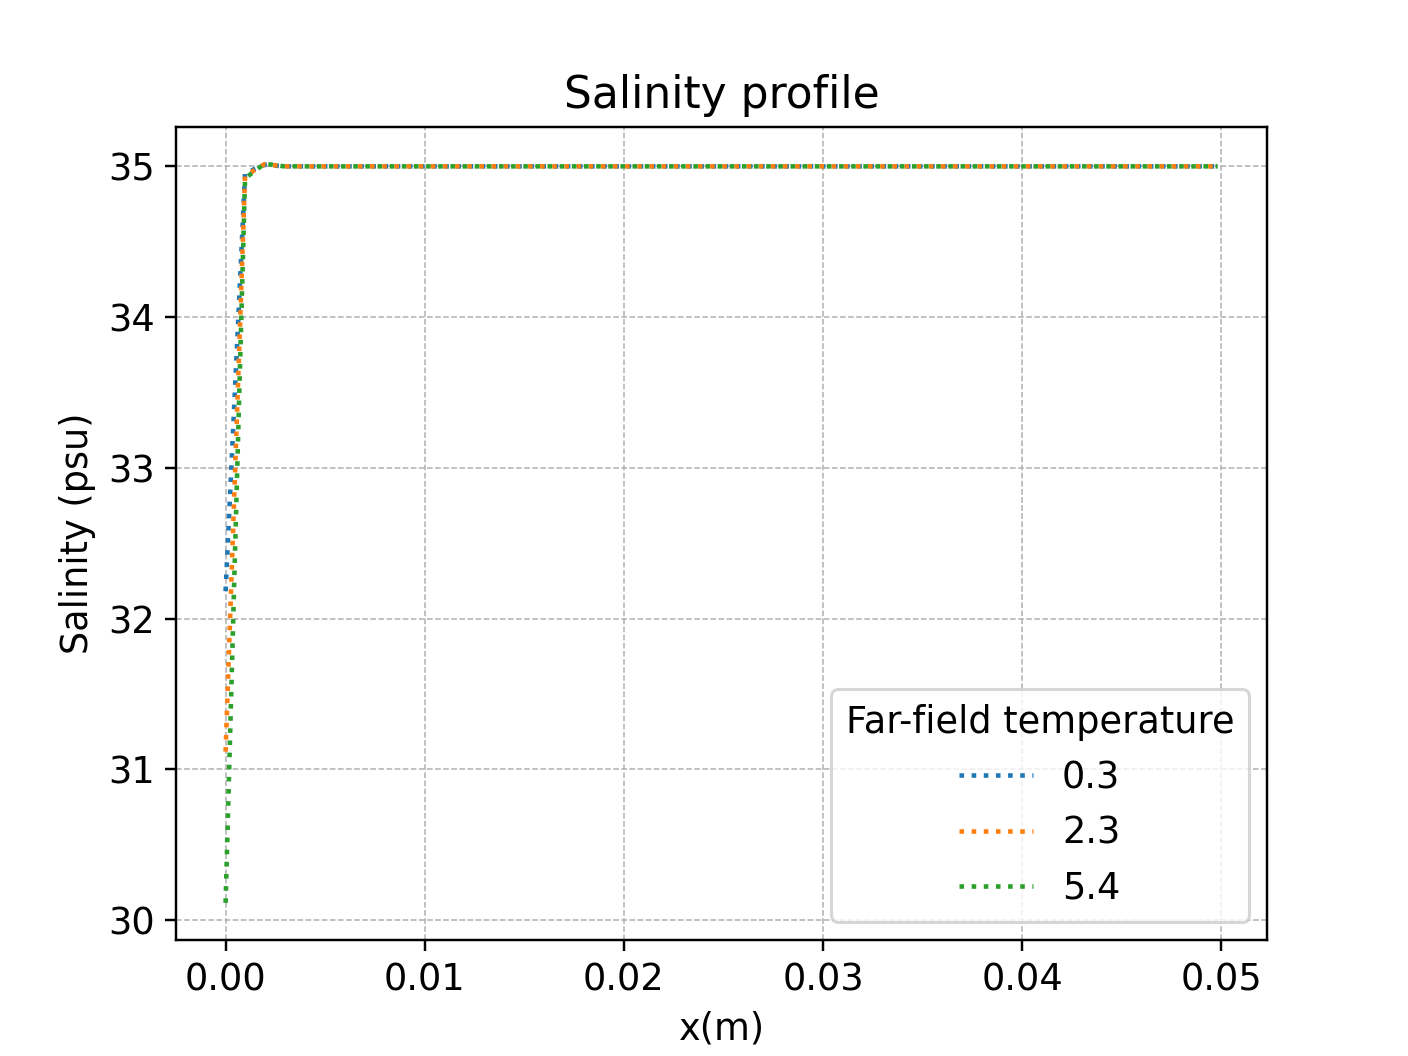
\includegraphics[width=12cm]{saltProfile}
	    \caption{Salinity profile}
	    \label{fig:3}
	\end{figure}
	
	Figure $\ref{fig:3}$ shows the behavior of the salinity near the ice face. Decreasing or increasing in the far-field temperature affects the interface region, and the sub-layers in temperature and salinity begin to grow. Examining the salinity profiles in figure $\ref{fig:3}$ and temperature profiles in $\ref{fig:2}$, the haline sub-layer grows slower than the thermal sub-layer due to t the larger molecular diffusivity of temperature.
	
	\subsection{Melt rate}
	
	\begin{figure}[H]
	    \centering 
	    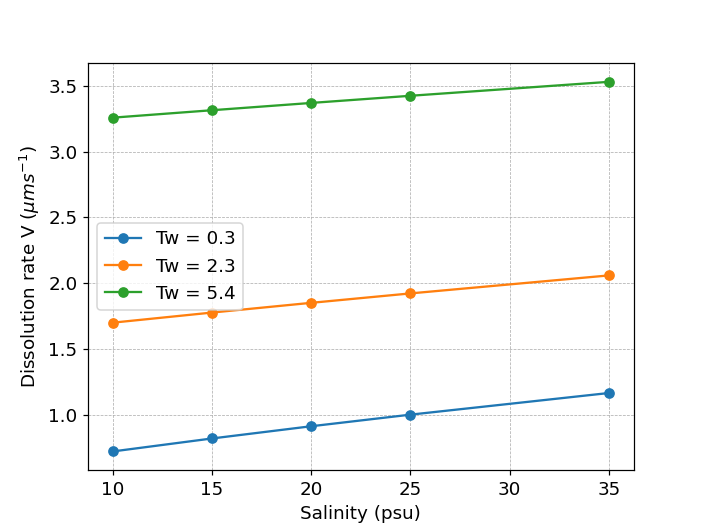
\includegraphics[width=12cm]{melt}
	    \caption{Melt rate at different ambient temperature}
	    \label{fig:4}
	\end{figure}
	
	Figure 5 depicts variations of the melt rate at different far-field temperatures (0.3, 2.3, and 5.4). It increases as the ambient temperature of the seawater increases. The results are reasonable because the larger far-field temperature enhances the heat transfer rate, increasing the melting rate. Similarly, increasing salinity at constant far-field temperature leads to an increase in melt rate. These results agree well with those produced in \citep{gayen2016simulation}. However, the melt rates in this work are higher, and this can be explained by the fact that we did not neglect the conduction within the ice $c_i \neq 0)$ and $T_b = a S_b+b+c p_b$. The increase in the melt rate as the salinity augment can be explained by the fact that a larger salinity leads to a larger salt diffusive flux at the interface and within the boundary layer. \cite{jenkins2011convection}), in their simulation with stratified ambient temperature, also found that the melt rate increases as the buoyancy and the sensible heat fluxes rise.
	
	%\subsection{Buoyancy flux}
	
	\section{Conclusion}
	
	
	
	
	
	
	\newpage
	
	%\bibliographystyle{unsrt}
	\bibliography{refComp}
\end{document}